% SPDX-FileCopyrightText: Copyright (c) 2021 Yegor Bugayenko
% SPDX-License-Identifier: MIT

\documentclass[landscape,slides,nodate,nosecurity]{/code/huawei.cls/huawei}
\usepackage[nocn]{ffcode}
\usepackage{/code/ssd16/slides}
\usepackage{clicks}
\usepackage{soul}

\renewcommand*\theauthor{Yegor Bugayenko}
\renewcommand*\thetitle{SIMBA}
\renewcommand*\thesubtitle{\textbf{Si}mplified \textbf{M}anagement \textbf{b}y \textbf{A}rtifacts}
\begin{document}

\plush[2]{
  \innoPin{
\includegraphics[width=\columnwidth]{simba-writing}}
  \innoMiddle{
    \innoTitle{\thetitle}{\thesubtitle}\par
    {\scshape\theauthor}\par
    \thecompany
  }
}

\plick{\innoHeader{Some Background:}}
\plick{I'm a head of an R\&D lab in Huawei MRC}
\plick{We invent tools to improve quality of code}
\plick{Our projects are R\&D, with a big \textbf{\large R}}
\plick{About 30 people in-house}
\plick{Nine teams/projects in five universities}
\plick{About 40 professors, postdocs, and students}
\plush{My role: to make sure projects don't fail}

\plick{\innoHeader{What Is Going On:}}
\plick{Most of them are pretty \textbf{smart},}
\plick{... \textbf{busy} with other projects (or teaching),}
\plick{... struggle to \textbf{decompose} research tasks,}
\plick{... \textbf{enjoy} the process,}
\plush{... and are very good \textbf{excuse-makers} :)}

\plick{\innoHeader{How We Managed Them Before:}}
\plick{Contract-based objectives}
\plick{Big milestones (3-4 months)}
\plick{Occasional meetings in Zoom}
\plush{A lot of trust, autonomy, and freedom}

\plick{\innoHeader{What We've Been Having:}}
\plick{A lot of reporting documentation}
\plick{Lack of practical results}
\plick{Missed deliveries}
\plush{Disappointment}

\plick{\innoHeader{Four Elements of SIMBA}}
\plick{1. Plan}
\plick{2. Monday Reports}
\plick{3. Status Calls}
\plush{4. Demos}

\plick{\innoSection{1. Plan}}
\plush{
  \innoPin{
\includegraphics[width=\columnwidth]{simba-thinking}}
  \begin{itemize}
    \item Dataset with 500+ files \br \textcolor{gray}{[Anna+Jeff, 3-Sep, 40\%]}
    \item XYZ module deployed \br \textcolor{gray}{ [John+Jeff, 14-Sep, 50\%]}
    \item Paper about data analysis \br \textcolor{gray}{ [Bill+Mary, 27-Sep, 20\%]}
    \item Survey conducted \br \textcolor{gray}{ [Jeff+Mary, 1-Oct, 0\%]}
    \item Technical report \br \textcolor{gray}{ [Mary+Anna, 5-Oct, 10\%]}
  \end{itemize}
}

\plick{\innoSection{2. Monday Report}}
\plush{
  \innoPin{
\includegraphics[width=\columnwidth]{simba-writing}}
  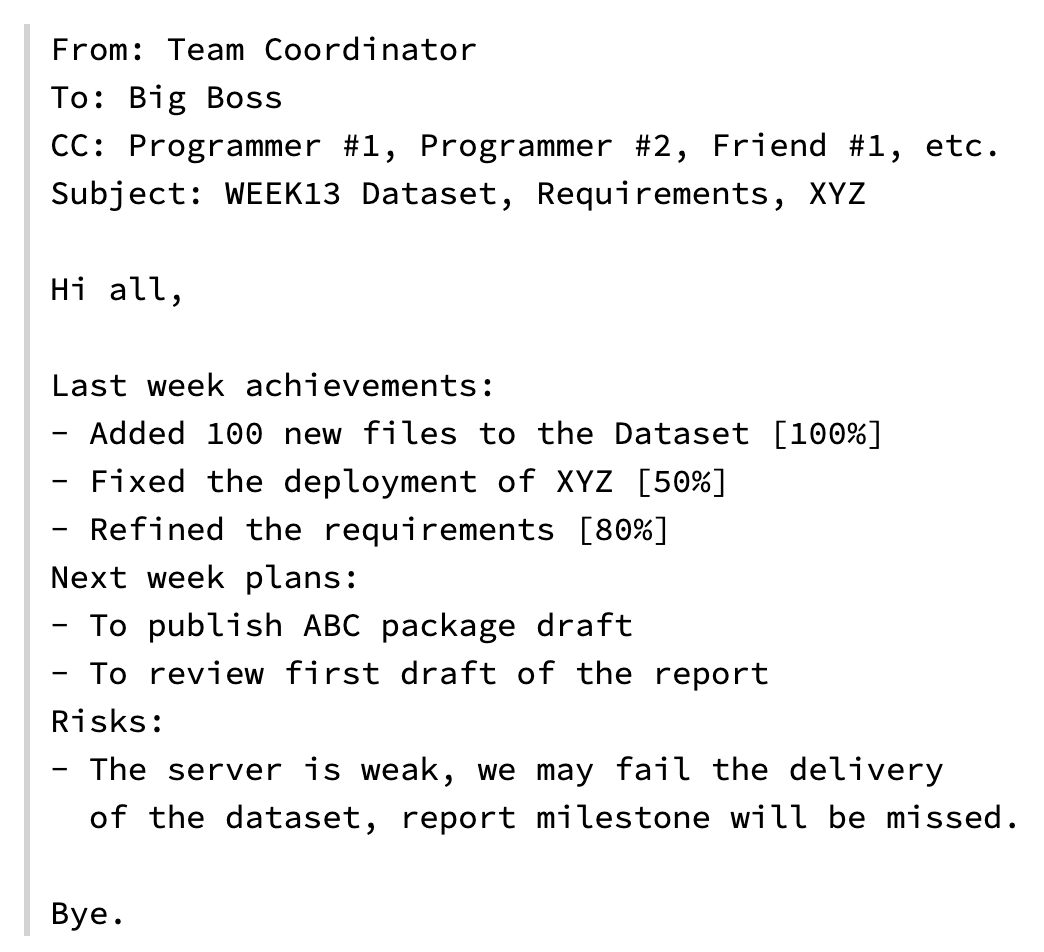
\includegraphics[width=0.6\columnwidth]{monday-report}
}

\plick{\innoSection{3. Weekly Call}}
\plush{
  \innoPin{
\includegraphics[width=\columnwidth]{simba-listening}}
  \begin{itemize}
    \item Will all artifacts delivered mean success?
    \item Did we break down the scope correctly?
    \item What did we miss in our Plan?
    \item All owners committed to the their artifacts?
    \item What are their intermediate committments?
    \item Are there any risks overlooked?
  \end{itemize}
}

\plick{\innoSection{4. Demos}}
\plush{
  \innoPin{
\includegraphics[width=\columnwidth]{simba-speaking}}
  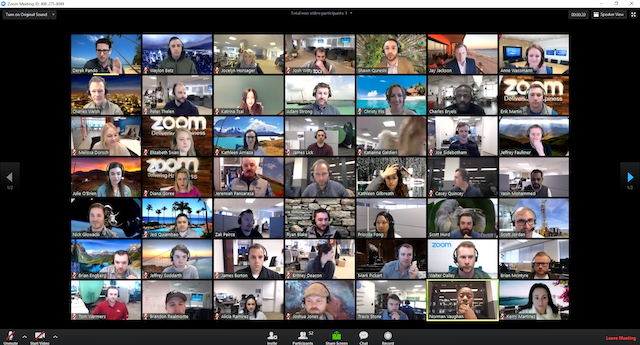
\includegraphics[width=0.6\columnwidth]{zoom-call}
}

\plick{\innoHeader{It's hard for everybody...}}
\plick{... to \textbf{decompose} research activities}
\plick{... to report \textbf{results} instead of actions}
\plick{... to stop making \textbf{excuses} at meetings}
\plush{... to talk about \textbf{risks} openly}

\plick{\innoThought{\raggedright Find me and follow on GitHub, Twitter, Instagram, LinkedIn, and Facebook: \textbf{@yegor256}\br\br Telegram: \textbf{@yegor256news}}}

\end{document}
